\documentclass[journal, a4paper]{IEEEtran}

\usepackage{graphicx}   % Written by David Carlisle and Sebastian Rahtz
                        % Required if you want graphics, photos, etc.
                        % graphicx.sty is already installed on most LaTeX
                        % systems. The latest version and documentation can
                        % be obtained at:
                        % http://www.ctan.org/tex-archive/macros/latex/required/graphics/
                        % Another good source of documentation is "Using
                        % Imported Graphics in LaTeX2e" by Keith Reckdahl
                        % which can be found as esplatex.ps and epslatex.pdf
                        % at: http://www.ctan.org/tex-archive/info/
\usepackage{color}
%\usepackage{psfrag}    % Written by Craig Barratt, Michael C. Grant,
                        % and David Carlisle
                        % This package allows you to substitute LaTeX
                        % commands for text in imported EPS graphic files.
                        % In this way, LaTeX symbols can be placed into
                        % graphics that have been generated by other
                        % applications. You must use latex->dvips->ps2pdf
                        % workflow (not direct pdf output from pdflatex) if
                        % you wish to use this capability because it works
                        % via some PostScript tricks. Alternatively, the
                        % graphics could be processed as separate files via
                        % psfrag and dvips, then converted to PDF for
                        % inclusion in the main file which uses pdflatex.
                        % Docs are in "The PSfrag System" by Michael C. Grant
                        % and David Carlisle. There is also some information
                        % about using psfrag in "Using Imported Graphics in
                        % LaTeX2e" by Keith Reckdahl which documents the
                        % graphicx package (see above). The psfrag package
                        % and documentation can be obtained at:
                        % http://www.ctan.org/tex-archive/macros/latex/contrib/supported/psfrag/

%\usepackage{subfigure} % Written by Steven Douglas Cochran
                        % This package makes it easy to put subfigures
                        % in your figures. i.e., "figure 1a and 1b"
                        % Docs are in "Using Imported Graphics in LaTeX2e"
                        % by Keith Reckdahl which also documents the graphicx
                        % package (see above). subfigure.sty is already
                        % installed on most LaTeX systems. The latest version
                        % and documentation can be obtained at:
                        % http://www.ctan.org/tex-archive/macros/latex/contrib/supported/subfigure/

\usepackage{url}        % Written by Donald Arseneau
                        % Provides better support for handling and breaking
                        % URLs. url.sty is already installed on most LaTeX
                        % systems. The latest version can be obtained at:
                        % http://www.ctan.org/tex-archive/macros/latex/contrib/other/misc/
                        % Read the url.sty source comments for usage information.

%\usepackage{stfloats}  % Written by Sigitas Tolusis
                        % Gives LaTeX2e the ability to do double column
                        % floats at the bottom of the page as well as the top.
                        % (e.g., "\begin{figure*}[!b]" is not normally
                        % possible in LaTeX2e). This is an invasive package
                        % which rewrites many portions of the LaTeX2e output
                        % routines. It may not work with other packages that
                        % modify the LaTeX2e output routine and/or with other
                        % versions of LaTeX. The latest version and
                        % documentation can be obtained at:
                        % http://www.ctan.org/tex-archive/macros/latex/contrib/supported/sttools/
                        % Documentation is contained in the stfloats.sty
                        % comments as well as in the presfull.pdf file.
                        % Do not use the stfloats baselinefloat ability as
                        % IEEE does not allow \baselineskip to stretch.
                        % Authors submitting work to the IEEE should note
                        % that IEEE rarely uses double column equations and
                        % that authors should try to avoid such use.
                        % Do not be tempted to use the cuted.sty or
                        % midfloat.sty package (by the same author) as IEEE
                        % does not format its papers in such ways.

\usepackage{amsmath}
\usepackage{listings}

\lstset{language=C} 



% Other popular packages for formatting tables and equations include:

%\usepackage{array}
% Frank Mittelbach's and David Carlisle's array.sty which improves the
% LaTeX2e array and tabular environments to provide better appearances and
% additional user controls. array.sty is already installed on most systems.
% The latest version and documentation can be obtained at:
% http://www.ctan.org/tex-archive/macros/latex/required/tools/

% V1.6 of IEEEtran contains the IEEEeqnarray family of commands that can
% be used to generate multiline equations as well as matrices, tables, etc.

% Also of notable interest:
% Scott Pakin's eqparbox package for creating (automatically sized) equal
% width boxes. Available:
% http://www.ctan.org/tex-archive/macros/latex/contrib/supported/eqparbox/

% *** Do not adjust lengths that control margins, column widths, etc. ***
% *** Do not use packages that alter fonts (such as pslatex).         ***
% There should be no need to do such things with IEEEtran.cls V1.6 and later.


% Your document starts here!
\begin{document}

% Define document title and author
	\title{JEThread: A Thread Pool Implementation in C}
	\author{Jialin Li and Edward Hu}
	\maketitle

% Write abstract here
\begin{abstract}
	JEThread is a Thread Pool written in C. It provides an easier interface and good performance for concurrent programming in C. JEThread achieves good performance across a mixture of workloads and automatically load balance through techniques like work stealing.
\end{abstract}

% Each section begins with a \section{title} command
\section{Introduction}
	% \PARstart{}{} creates a tall first letter for this first paragraph
	\PARstart{T}{hread} is a basic unit of CPU utilization, it consists of program counter, register set, and its own stack. Compared to processes, threads are much more lightweight since virtual memory space remains the same during a thread switch, which is not true for process switch. However, even threads sometimes pose overhead that will affect the performance of the program. Initializing and cleaning threads can pose a certain amount of overhead. For a concurrent application that creates and destroys a large number of threads that each only runs for a short time, the thread management mechanism can cause unnecessary resource waste. Thread pool can be useful in this type of scenario as it reduces the complexity of thread management and the overhead involved in thread creation and cleaning. 

% Main Part
\section{Background}	
	Without a thread pool, the common techniques used to do concurrent programming in C are to spawn a thread for each task, if task is long running, or to create a fixed number of worker threads and statically partition the work among the workers. Although both ways are feasible and provide control freedom to programmers, they can also be unnecessary burdens and require programmers to have a great deal of knowledge of both the workloads they are running and the type of thread programming model that  would result in good performance. Newer languages like Golang deals with this problem by providing Goroutines which are extremely lightweight user threads, as well as other concurrent native objects to better support concurrent programming. These features have brought Golang many users. For example, container engines like Docker and LXD, container orchestration tools like Kubernetes are all written in Golang. While it is hard to fully integrate runtime concurrent programming support in C, the thread pool abstraction provides a good middle ground.
		

\section{Motivation}
	Our primary goal is to implement a thread pool that is easy to use and flexible with different workloads. We minimizes the number of functions in the thread pool interface to keep it narrow yet fully functional. We also make a distinction between blocking and nonblocking tasks, and adopt techniques like work stealing to support various workloads.
	We also want the thread pool to be reasonably more performant than previously mentioned pthread-based approaches. Thus we create several test cases to compare the performance in different implementations. Finally, we simply want to learn the inner-working of an efficient thread pool and explore the drawbacks along with possible improvements.\\
	
\section{Programming Interface}
The programming interface is designed for simplicity, there are three functions users are exposed to.\\

\begin{itemize}
	\item \begin{lstlisting}
void thread_pool_init(int workers, 
		      int mutex_flag);
	\end{lstlisting}
	This function initializes a new thread pool. The \textbf{workers} attribute specifies the number of threads that can exist in a thread pool. If $0$ is passd in, the number of threads will be initialized to the number of core in the execution environment. The \textbf{mutex\_flag} argument let user decides whether to use mutex or spinlock as synchronization method. Note if the thread pool is initialized more than once, every invocation of this function will be discarded.\\
	\item 
	\begin{lstlisting}
bool thread_pool_add(task_func *func,
		     void* aux,
		     enum CallType);
	\end{lstlisting}
	This function adds tasks to the thread pool. The \textbf{func} attribute represents the function that is to be executed. The \textbf{aux} attribute indicates the parameter \textbf{func} takes in. the \textbf{CallType} specifies whether to use blocking or non-blocking mechanism for the thread pool. If a task is added without failure, $true$ is returned. Otherwise, $false$ will be returned.\\
	\item \begin{lstlisting}
void thread_pool_wait();
	\end{lstlisting}
	This function blocks until all threads in thread pool have finished all the existing jobs.
		\end{itemize}

\section{Implementation}
The low overhead of the thread pool is achieved with several design decisions. We will discuss the major implementations. 
\subsection{Task Assignment}
Each task is represented as a \textbf{struct task}. It is created by the calling function whenever the user sends the function to be executed to the thread pool and then distributed to the threads in the thread pool in a round-robin style to ensure even distribution. We keep track of the current worker that we are assigning to, and advance it after we've assigned $N$ tasks to it. This is to reduce the overhead of waking up workers when the number of tasks is few, and to try batching tasks and provide better tasks locality. This is based on the hypothesis that tasks created close in time are likely to reference similar memory regions. Therefore, we hope to keep them on the same worker thread. Even when this hypothesis does not hold, it does not hurt JEThread's performance. When a job is assigned to a worker, the main thread grabs the lock(spinlock suggested) to the worker's private queue and add it to the queue.

\subsection{Blocking versus Non-Blocking Tasks}
In addition to batch assigning jobs, we also treat blocking and nonblocking tasks differently. This is necessary because JEThread by default starts with $N$ threads, where $N$ is the number of processors, and if all workers threads are executing some blocking tasks, then nonblocking tasks will not be able to execute until much later. It becomes even worse when majority of tasks are blocking tasks. In such case, the fixed number of workers would be blocked constantly. To solve this problem, we use an approach similar to Golang's parking threads, where we create a new thread to handle blocking tasks and only use our default set of worker threads to handle nonblocking tasks. In order to implement this, we need to identify if a task is blocking or nonblocking. This is difficult and inefficient to do at runtime, but can be done much easier in compile time. In our implementation, we rely on user to specify the CallType when adding a task. This is not fundamentally necessary - we could have modified GCC compiler or inspected task at preprocessing time to accomplish the same thing, but due to the time constraint we exposed this option to users. We believe that users would try their best to provide accurate CallType because they want better performance. Even if they accidentally misidentified CallType, this would not effect the correctness of JEThread.

\subsection{Work Stealing}
One of our goals is to achieve automatic load balancing. For this purpose, we implement work stealing for each worker thread. For each worker, we first do a sem\_trywait() to see if there is any job on its private queue. If there is none, then it randomly selects a victim thread and tries to steal a task from the victim and executes it. If keeps doing so until there is no more work to steal or if it has stolen $N$ times, where $N$ is the number of workers. This is our first attempt at work stealing. To optimize this, we could have kept randomly selecting victims until there is a victim with work above a certain threshold or up to a certain number of tries. To avoid all workers trying to steal when there is no tasks available, we can also use randomization to determine if a worker should try work stealing or just block until it is assigned a job. Another optimization we can perform is to steal more than one work at a time since we want it to be worth the overhead of running the algorithm. Although not reflected in the evaluation, we did try to evaluate the impact of the current work stealing techniques and found that even the naive approach improves JEThread's performance slightly.

\subsection{Internal Synchronization}
Each thread owns a privat task queue to store all its assigned tasks. Each queue is protected by either a mutex or a spinlock depending on users' specification. However, it is possible that a thread's task queue is empty when it is first initialized. It will waste CPU resource if such task is kept up and running without executing any tasks. Thus, we use semaphore to improve the efficiency of the thread pool. Thus we let the main thread invoking sema\_post on each thread once it finishes adding tasks to the thread's task queue to indicate the availability of tasks. However, the thread's task queue can be empty for other reasons. The most important one is that the thread finishes executing all assigned tasks. Thus, we implement work stealing algorithm to keep the idle thread busy by letting it trying to steal tasks from other threads by randomly choosing one. Since we don't want tasks stealing to create too much overhead as it tries to grab tasks from other threads, we simply let the idle thread using pthread\_mutex\_trylock() or pthread\_spin\_trylock(). If the stealing succeeds, the tasks is grabbed from the victim's task queue and executed. Otherwise, the steal will fail. If the steal fails too many times, that indicates many threads' task queue is already empty and the thread pool is getting close to running out of tasks. In this case, letting more threads trying to steal tasks will create unnecessary overhead, thus the thread will be blocked to prevent wasting resources. If eventually the threads run out of tasks, it will increase \textbf{wait\_sema} to let the main thread know it finishes its job. If all threads signify that they've finihsed their tasks, then thread pool is terminated.

\section{Evaluation}
Below is the hardware we used to conduct experiements on the performance of the thread pool.
	\begin{table}[!hbt]
		% Center the table
	\begin{center}
		\caption{Hardware Sepcification}
		\label{tab:simParameters}
		% Table itself: here we have two columns which are centered and have lines to the left, right and in the middle: |c|c|
		\begin{tabular}{|c|c|}
			% To create a horizontal line, type \hline
			\hline
			% To end a column type &
			% For a linebreak type \\
			Processor & Intel® Core™ i7-6700 CPU \\
								&@3.40GHz $\times$ 8\\
			\hline
			RAM & $15.6$ GiB \\
			\hline
			OS & Ubuntu 16.04.4 LTS 64-bit\\
			\hline
			Compiler & GCC 5.40\\
			\hline
		\end{tabular}
		\end{center}
	\end{table}
	
There are several goals we are aiming to achieve in the experiment. First, we want to run both long and short tasks in the threal pool to analyze which type of tests have the most impact on the performance on the program. We've created created various tests for the thread pool to perform and we will show the data collected later in the analysis section. We hope the low overhead of switch between tasks will help us outperform thread-based implementation as well go-based implementation. In addition, we implemented work stealing mechanism to improve the work throughput done by the thread pool. We hope the work stealing function will further improve the efficiency of the thread pool. 	
	

We create same tasks for every implementation to execute to ensure fairness. we've selected three types of tests that represent three typical scenarios in most applications. We designed a task that accesses file system and performs read and write operations. Since accessing file system usually requires blocking which generates large overhead, this task is perfect to represent tasks that takes more than a few CPU cycles to finish. We also designed a task that task an argument, and then computer then sum based on the input and generates a simple hash value. This represents a short to medium tasks present in most applications and we selected it as a candidate to represent short tasks. We also include a task that does nothing in order to test sheer performance of the thread pool without the influence of any outside factors. In addition, we mixed the number of long and shorts tasks in each benchmark in order to generalize the real life scenario where a mixture of different tasks are executed. We want to show that the speedup is not or at least minimally affected by the type of tasks executed. Then, we test the scalability of the thread pool itself by gradually increase the number of threads in the thread pool running $10,000$ tasks. The result matches with our expectation as the scalability is achieved when increasing the number of threads in the thread pool.\\

\newpage

\begin{figure}[!hbt]
		% Center the figure.
		\begin{center}
		% Include the eps file, scale it such that it's width equals the column width. You can also put width=8cm for example...
		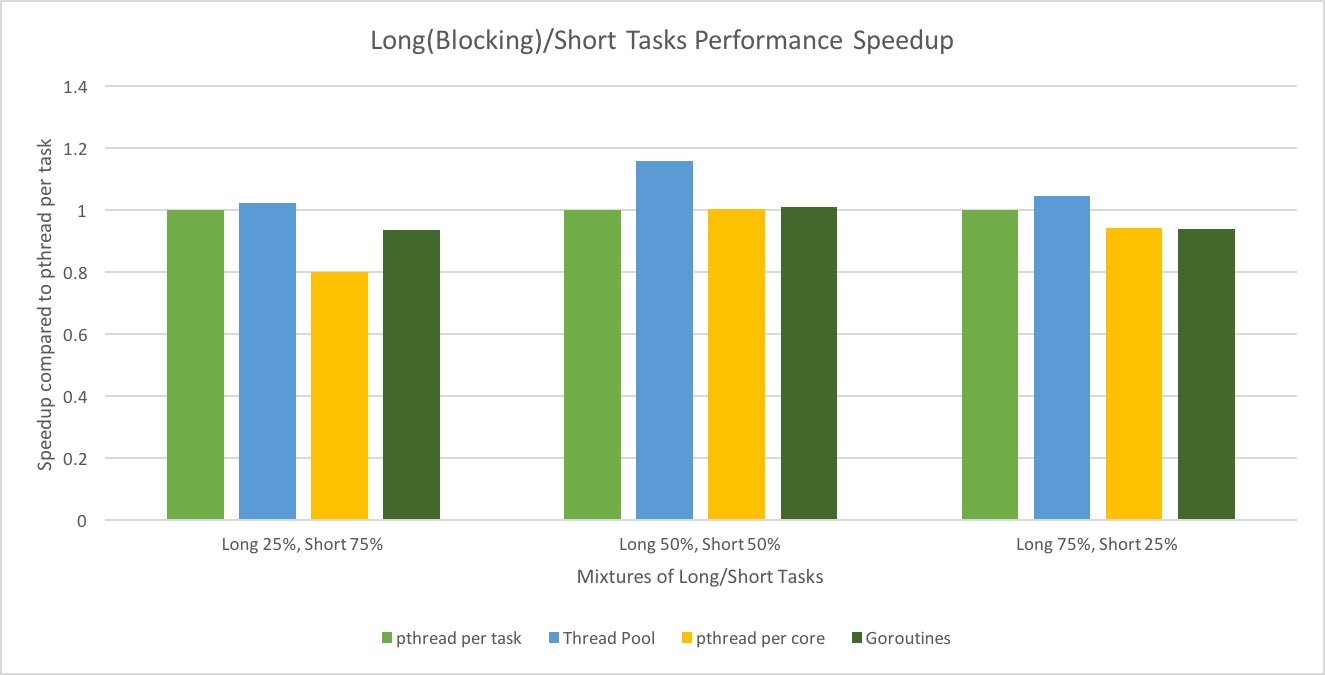
\includegraphics[width=\columnwidth]{test_1.png}
		% Create a subtitle for the figure.
		\caption{Benchmark speedup using long blocking tasks and short tasks. From left to right each section represents: long 25\% with short 75\%, long 50\% with short 50\%, and long 75\% with short 25\%. Green bar: pthread per task. Blue: Thread pool. Yellow: pthread per core. Dark Green: Goroutines}
		% Define the label of the figure. It's good to use 'fig:title', so you know that the label belongs to a figure.
		\label{fig:tf_plot}
		\end{center}
	\end{figure}
	
	
\begin{figure}[!hbt]
		% Center the figure.
		\begin{center}
		% Include the eps file, scale it such that it's width equals the column width. You can also put width=8cm for example...
		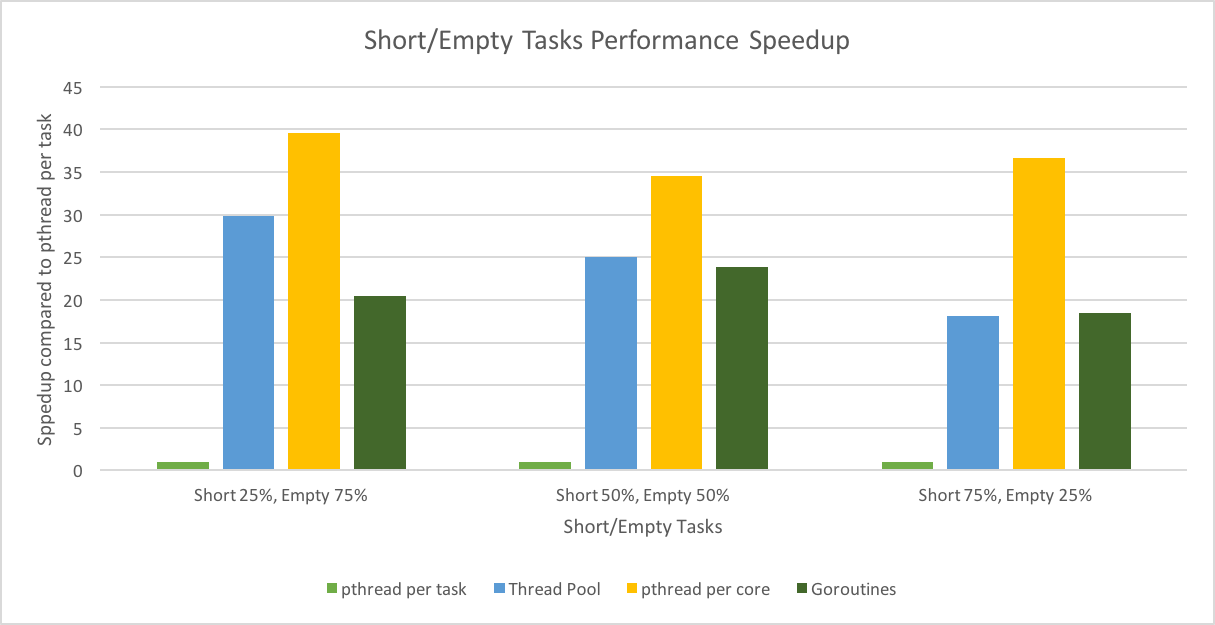
\includegraphics[width=\columnwidth]{test_2.png}
		% Create a subtitle for the figure.
		\caption{Benchmark speedup using short blocking tasks and empty tasks. From left to right each section represents: long 25\% with short 75\%, long 50\% with short 50\%, and long 75\% with short 25\%. Green bar: pthread per task. Blue: Thread pool. Yellow: pthread per core. Dark Green: Goroutines}
		% Define the label of the figure. It's good to use 'fig:title', so you know that the label belongs to a figure.
		\label{fig:tf_plot}
		\end{center}
	\end{figure}
	
\begin{figure}[!hbt]
		% Center the figure.
		\begin{center}
		% Include the eps file, scale it such that it's width equals the column width. You can also put width=8cm for example...
		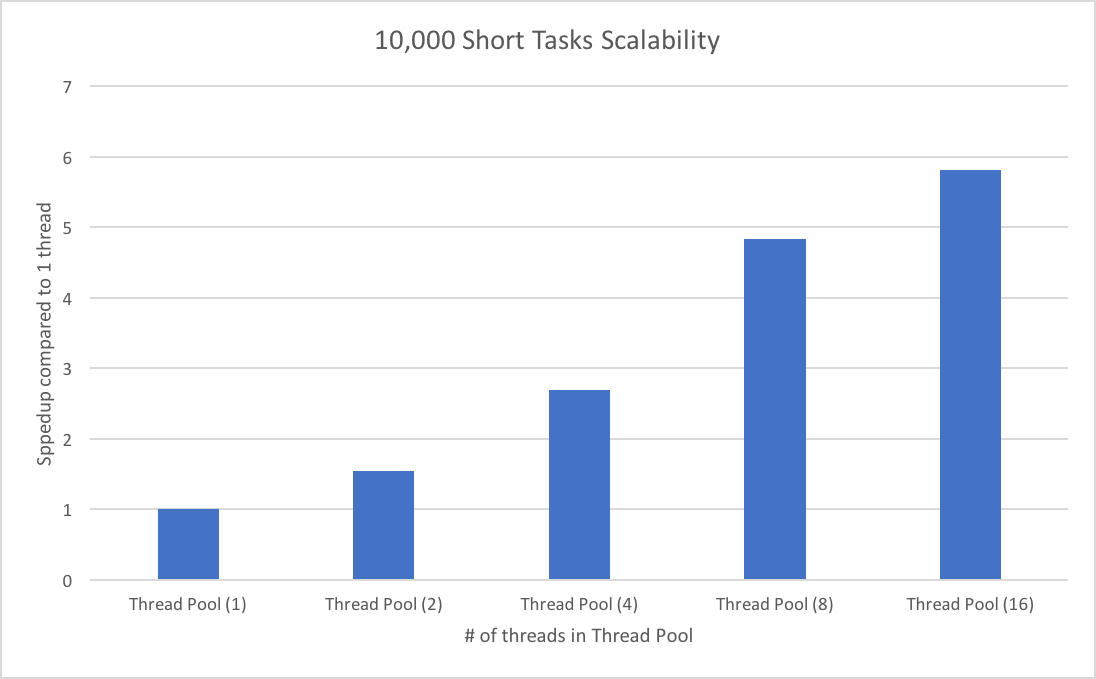
\includegraphics[width=\columnwidth]{test_3.png}
		% Create a subtitle for the figure.
		\caption{Benchmark scalability of thread pool with $10,000$ tasks running. Threads used from left to right: $1$, $2$, $4$, $8$, $16$.}
		% Define the label of the figure. It's good to use 'fig:title', so you know that the label belongs to a figure.
		\label{fig:tf_plot}
		\end{center}
	\end{figure}

\section{Conclusion}
	Theoratically, thread pool can be very efficient especially dealing with a large number of relatively short tasks concurrently. In order to acheive maximum performance boost, the use of context switch should be minimized. The thread pool does a greate job of reducing the overhead in context switch. In addition, work stealing further facilitates the work throughput by letting idle threads execute other threads' tasks. However, thread pool is not a silver bullet that solves every problem of thread. The overhead of thread context switch is transfered to each thread's task queue as executing tasks requires dequeing the task each time, which also applies to job stealing. We've also conducted experiement with creating only one task queue shared between all threads, but the same thing still applies here that the overhead is transfered to the queue since accessing tasks is performed with lock's protection. In addition, round-robin style task distribution may not be the best way to distribute tasks as calling thread is unware of the actual workload in its distribution target. The work stealing is also very tricky to implement as the stealer is not aware of the workload distribution during runtime. If the majority of threads finish execution while a few survivor threads with many tasks are still alive, the parallelism can be compromised since a few threads become the bottleneck that causes main threads waiting unnecessarily. Additional improvements such that runtime dynamic workload check and compiler support for user-guided optimization will further increase the usibility of thread pool.\\
	
	In summary, the thread pool is great for running a large amount of tasks effciently with relatively small number of threads. In parallel applications with many short tasks to perform thread will be a strong candidate solution.

% Your document ends here!
\end{document}